\chapter{Motor Learning in Virtual Reality}
(5 pages)

\section{Motor Learning}
grundlagen des motor learning
\section{Visual Perspectives}

\begin{figure}[htb]
	\centering
	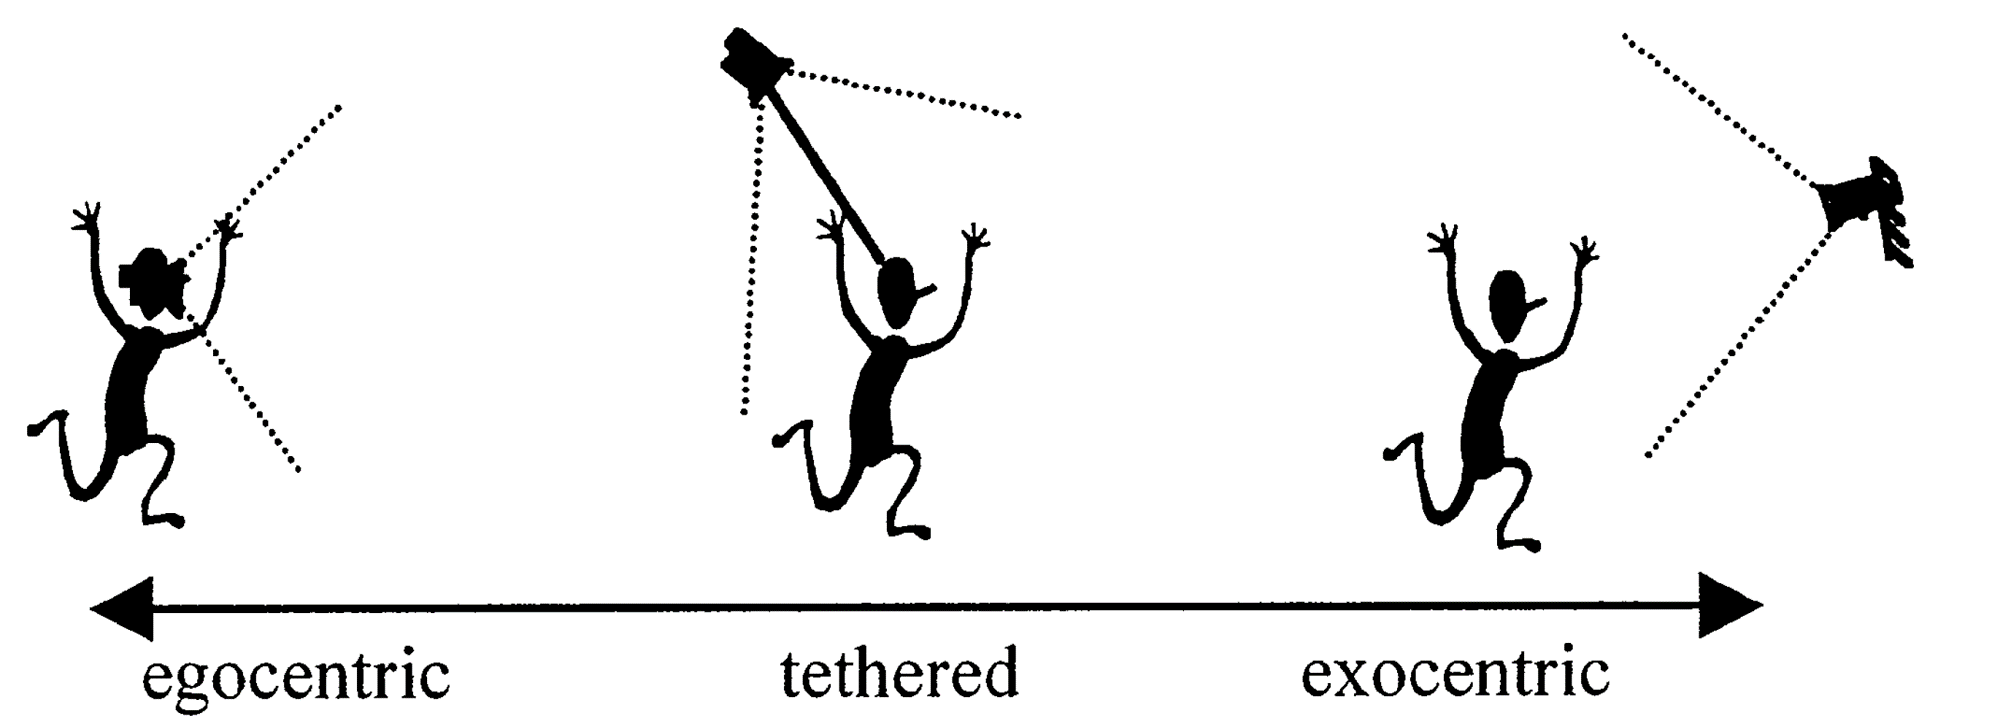
\includegraphics[width=\textwidth]{figures/ego_exo_continuum.PNG}
	\caption[Ego-Exo continuum by Milgram]{Ego-centric / exo-centric continuum by Milgram \todo{source}}
	\label{fig:ego-exo-continuum}
\end{figure}

\begin{figure}[htb]
	\centering
	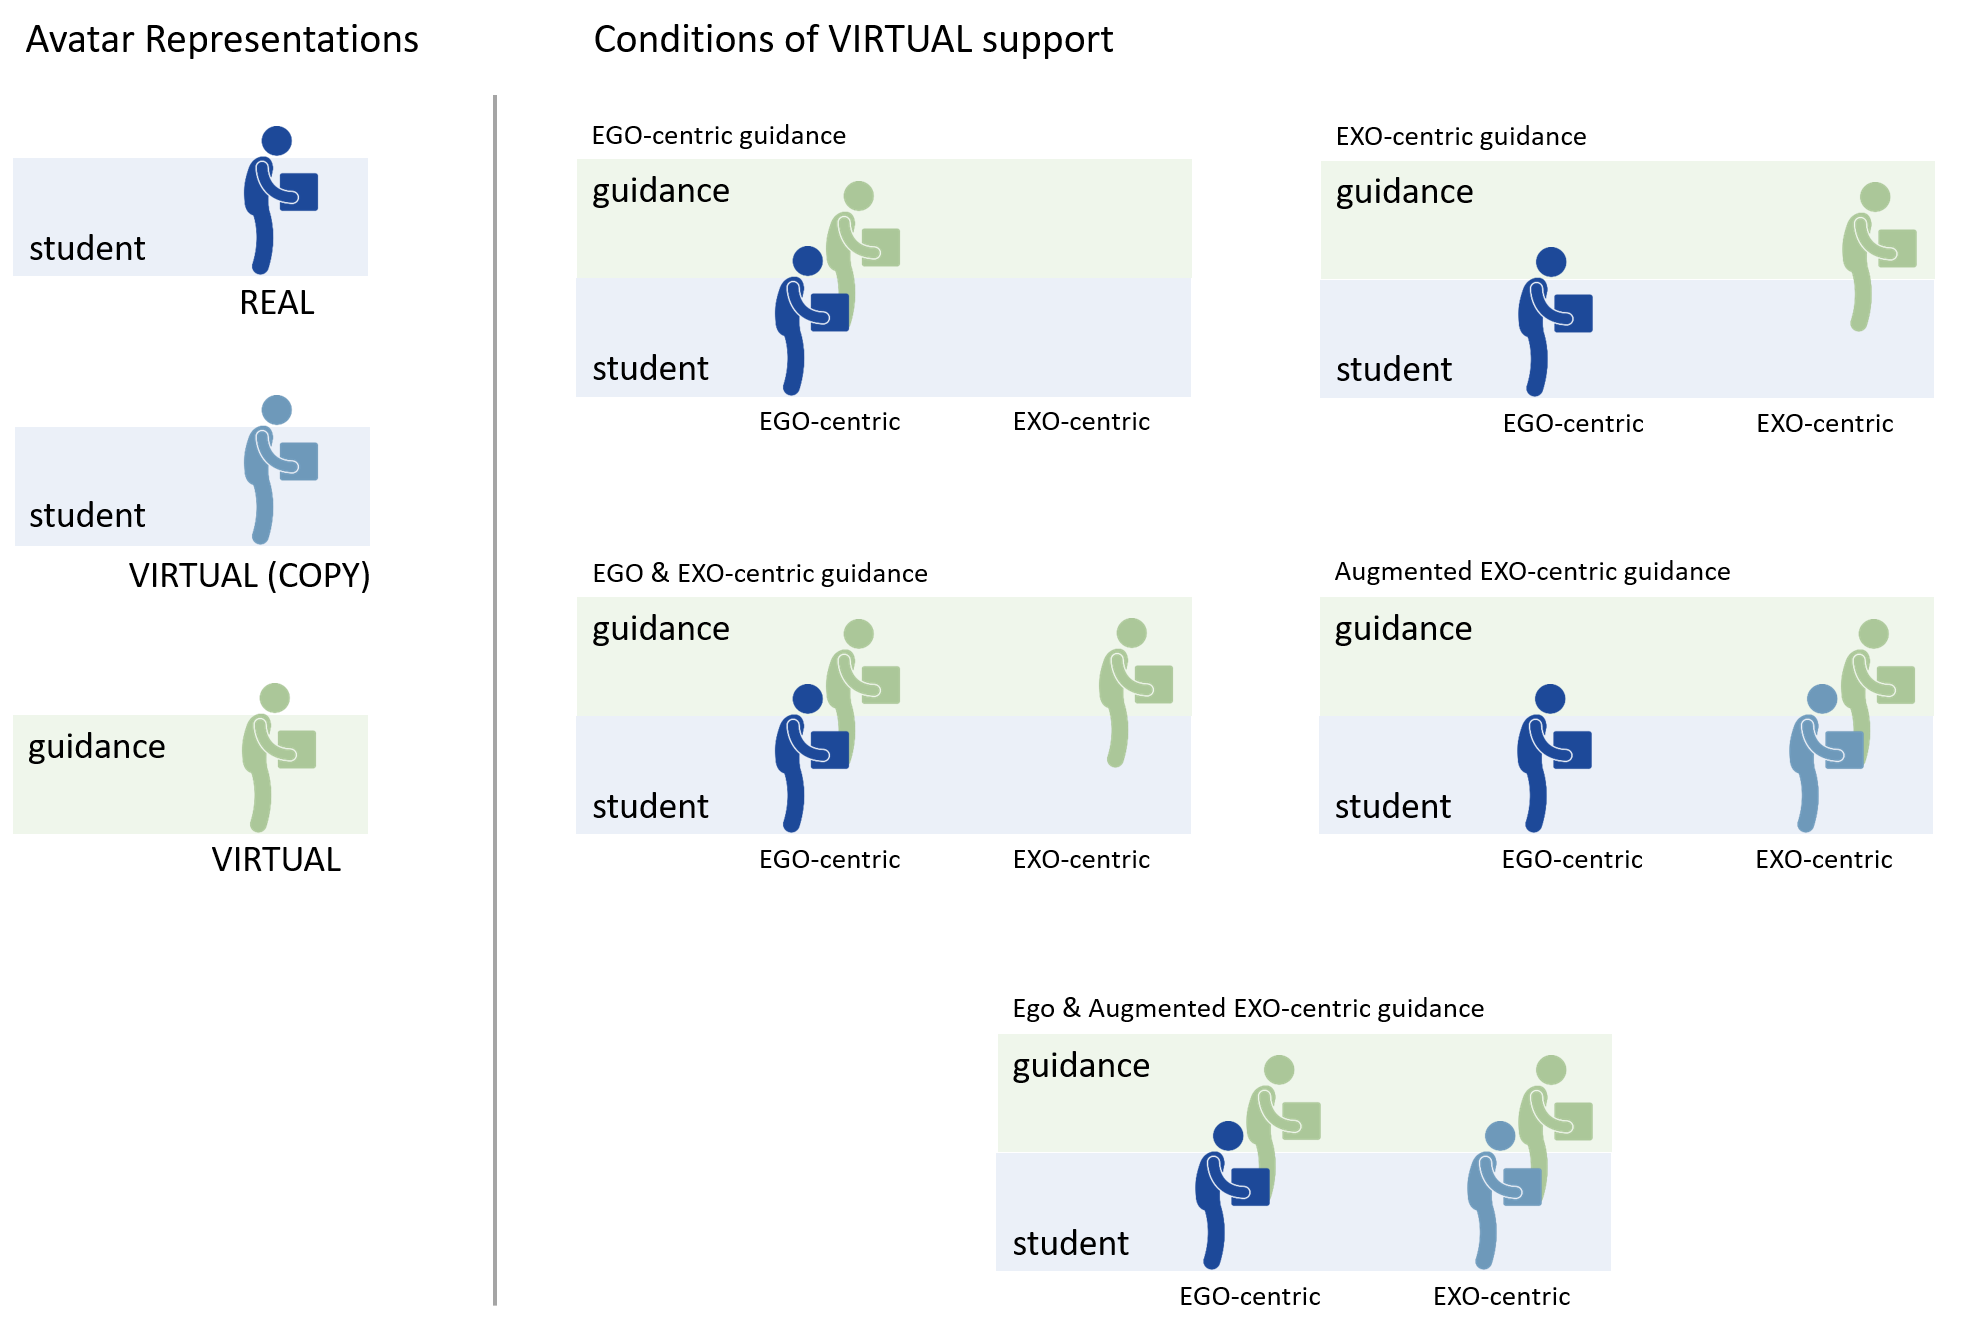
\includegraphics[width=\textwidth]{figures/perspectives.png}
	\caption[Possible perspectives]{Possible perspectives with one real world student and one real world teacher.}
	\label{fig:perspectives}
\end{figure}

\begin{figure}[htb]
	\centering
	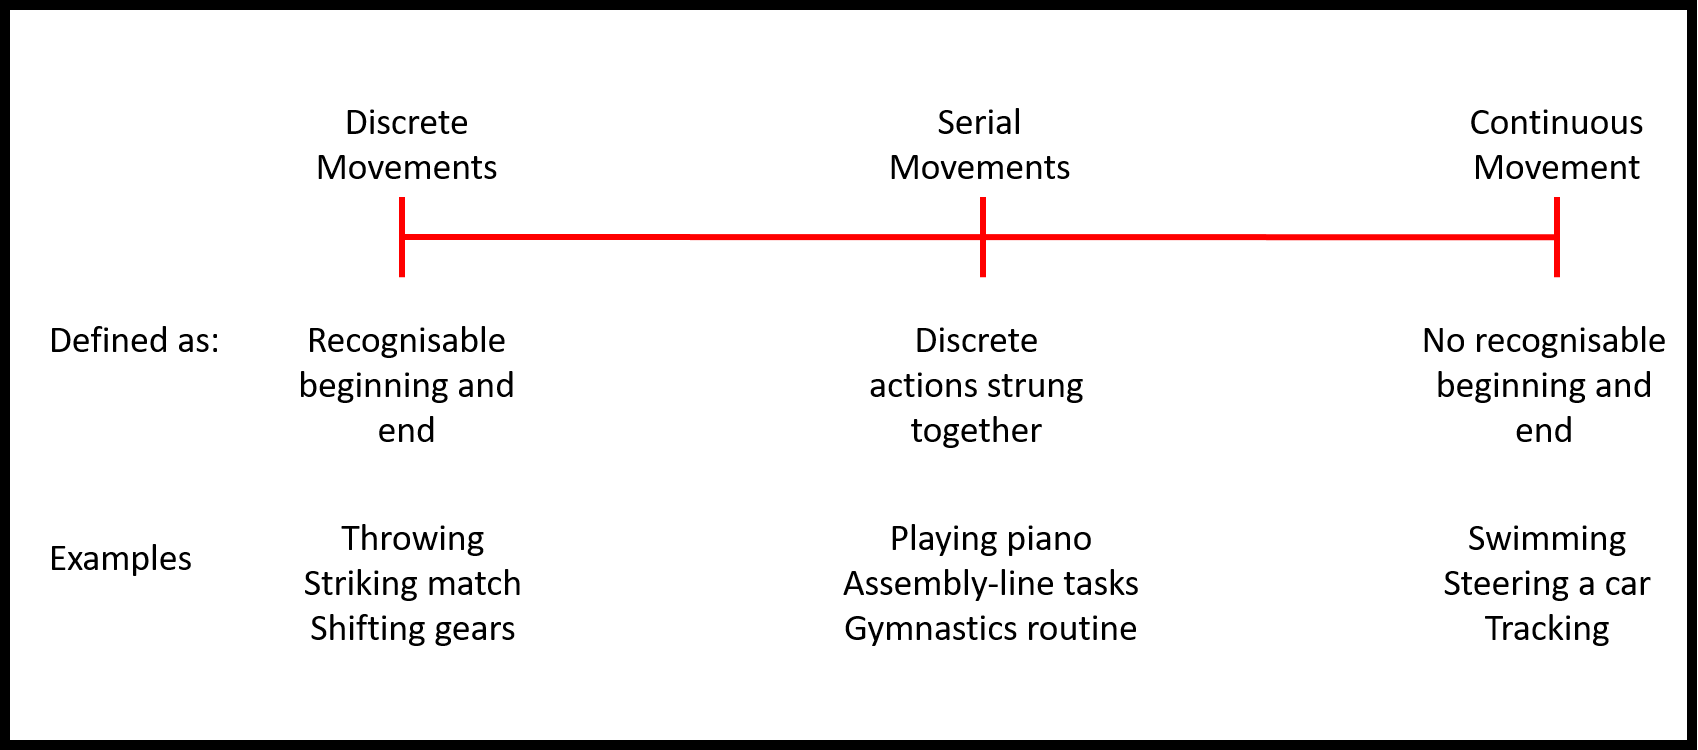
\includegraphics[width=\textwidth]{figures/movement_classification.png}
	\caption[Movement classification 1]{Movement classification 1}
	\label{fig:movement_classification}
\end{figure}

\begin{figure}[htb]
	\centering
	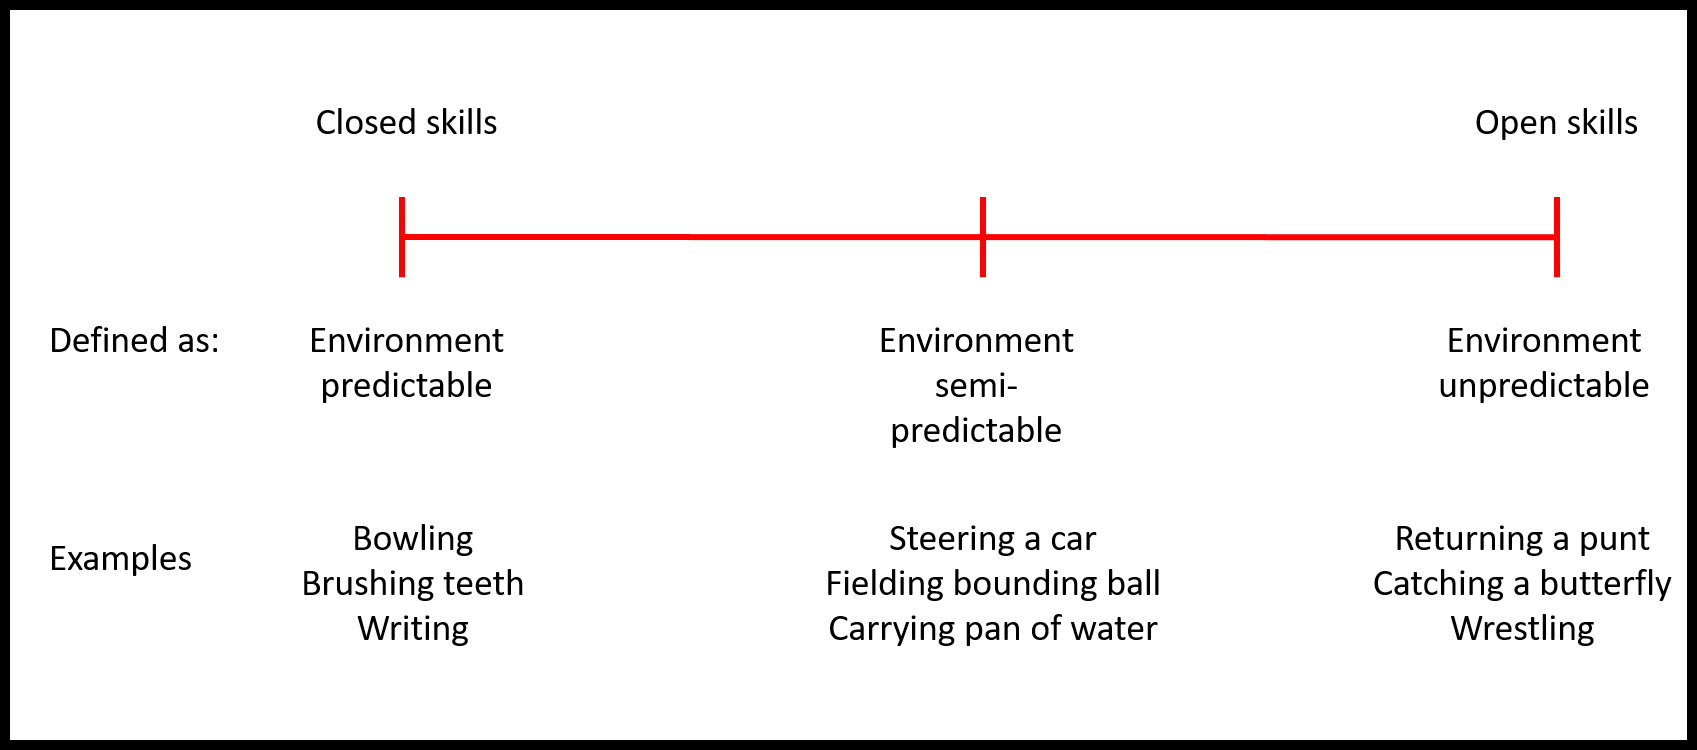
\includegraphics[width=\textwidth]{figures/movement_classification2.png}
	\caption[Movement classification 2]{Movement classification 2}
	\label{fig:movement_classification2}
\end{figure}

ego-exo continuum,
\section{measurements for motorlearning?}
\section{Mixed Reality}
\begin{figure}[htb]
	\centering
	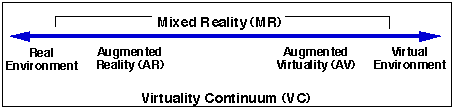
\includegraphics[width=\textwidth]{figures/milgram_continuum.png}
	\caption[Ego-Exo continuum by Milgram]{Ego-centric / exo-centric continuum by Milgram \todo{source}}
	\label{fig:mr_continuum}
\end{figure}


argumentation warum VR und nicht AR?
\section{Motorlearing in Virtual Reality}
\begin{figure}[htb]
	\centering
	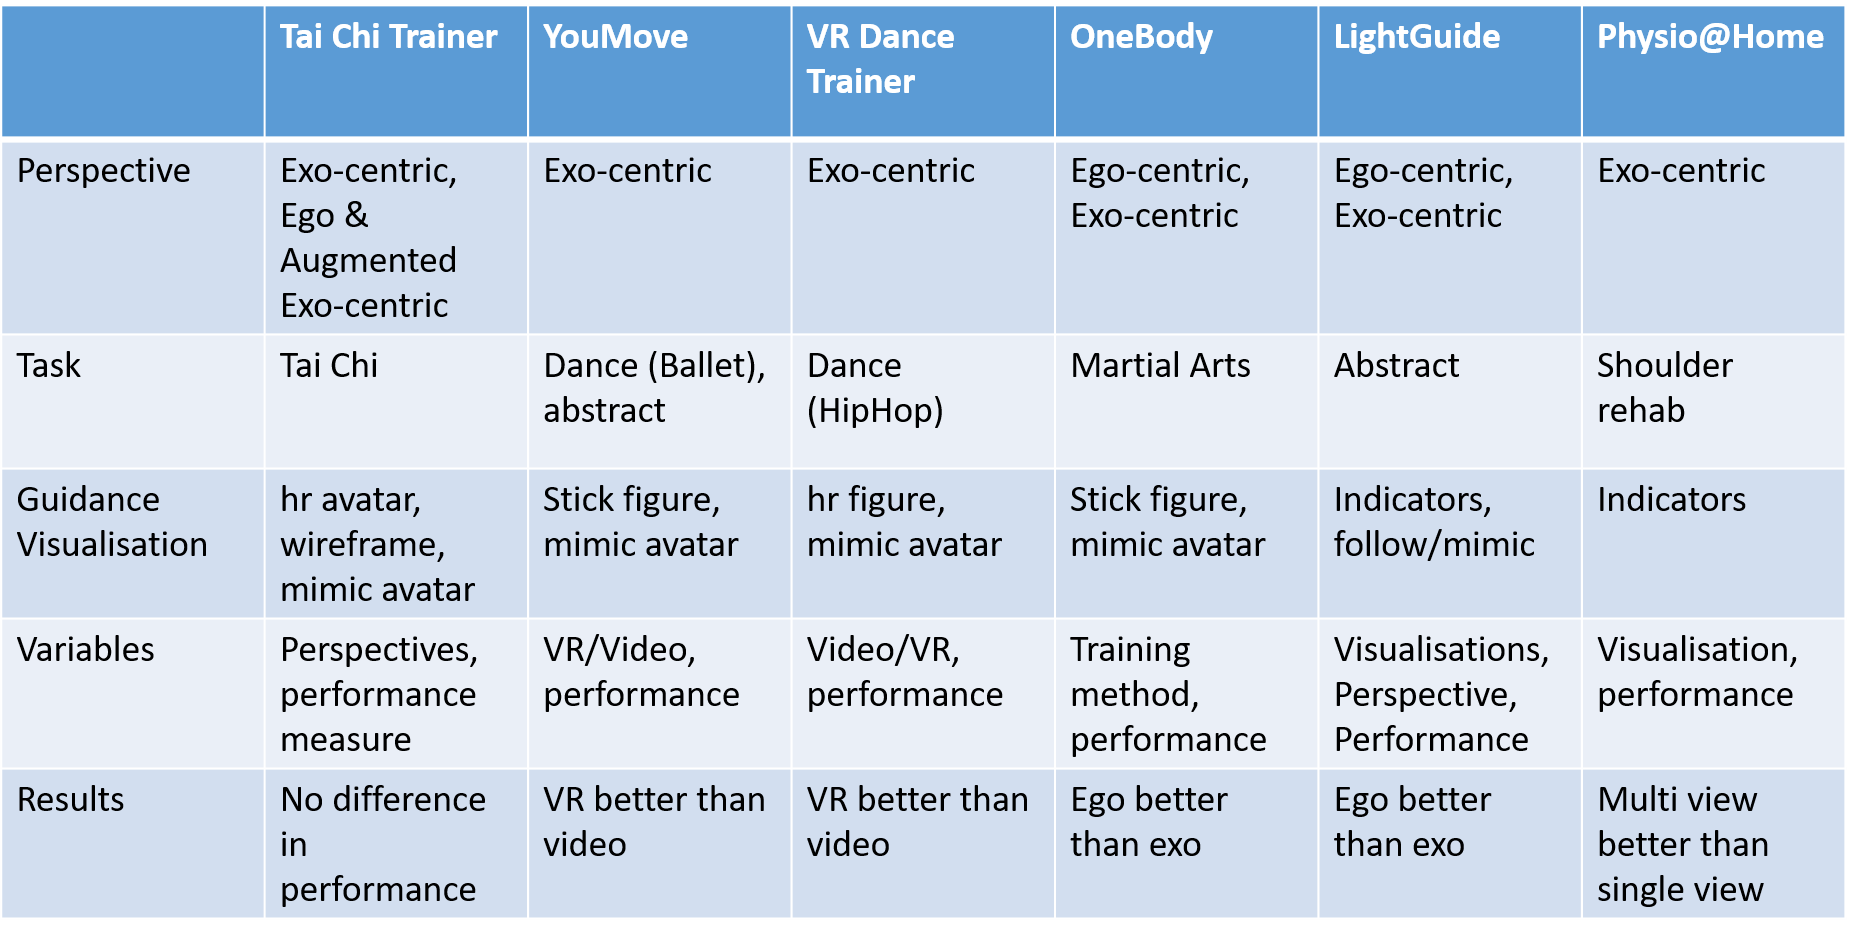
\includegraphics[width=\textwidth]{figures/detail_paper_overview.png}
	\caption[Overview seminar evaluation]{Overview seminar evaluation}
	\label{fig:rw_overview_detail}
\end{figure}

\begin{figure}[htb]
	\centering
	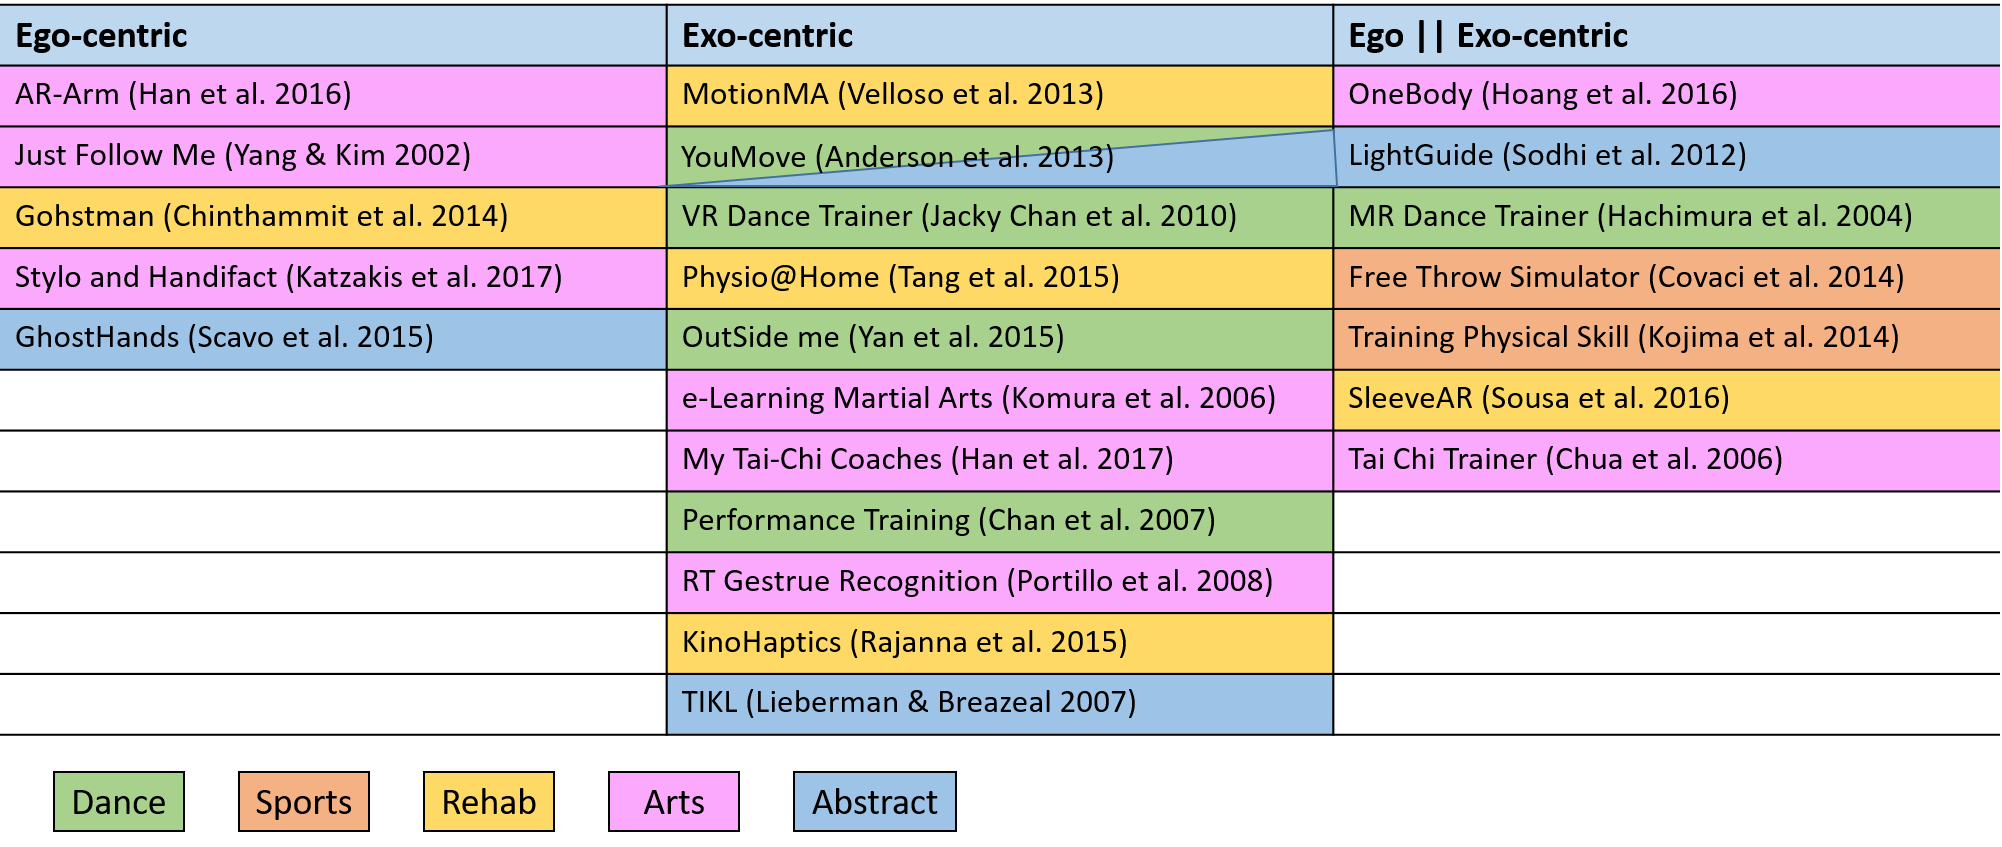
\includegraphics[width=\textwidth]{figures/rw_overview.png}
	\caption[Overview seminar evaluation]{Overview Related Work divided by perspective and task}
	\label{fig:rw_overview}
\end{figure}
bekannte arbeiten und deren ergebnisse über motor learning in VR\\
\\
auf basis dieses kapitels wird die studie geformt

